\documentclass[11pt]{article}

\usepackage[letterpaper,margin=0.75in]{geometry}
\usepackage{booktabs}
\usepackage{caption}
\usepackage{graphicx}
\usepackage{listings}
\usepackage{float}
\usepackage{scrextend}
\usepackage{hyperref}
\usepackage[parfill]{parskip}
\renewcommand{\lstlistingname}{Snippet}


\begin{document}

\lstset{
  language=Python,
  basicstyle=\small,          % print whole listing small
  keywordstyle=\bfseries,
  identifierstyle=,           % nothing happens
  commentstyle=,              % white comments
  stringstyle=\ttfamily,      % typewriter type for strings
  showstringspaces=false,     % no special string spaces
  numbers=left,
  numberstyle=\tiny,
  numbersep=5pt,
  frame=tb
}

\title{Congestion Control Part 1}

\author{Brandt Elison & Joe Eklund}

\date{March 16, 2016}

\maketitle

\section{Introduction}

For this project we implemented the slow start, additive increase, and multiplicative decrease elements of TCP Tahoe congestion control algorithm. The following tests were used to verify that we correctly implemented the different elements of the algorithm.

Each test resulted in a sequence plot, which shows packets and ACKs sent and received over time. The y axis represents the packet number modulo 50. The modulo 50 simply prevents the plots from being unreasonably tall. The x axis represents time in seconds. The boxes on the graph represent packets transmitted by the sender, and the dots represent ACKs received by the sender. Each X represents a lost packet.

\section{Test Results}


\begin{enumerate}
  \item Slow Start
  
\begin{figure}[H]
\caption{The graph of our slow start test output.}
	\label{figure1}
  	\centering
  	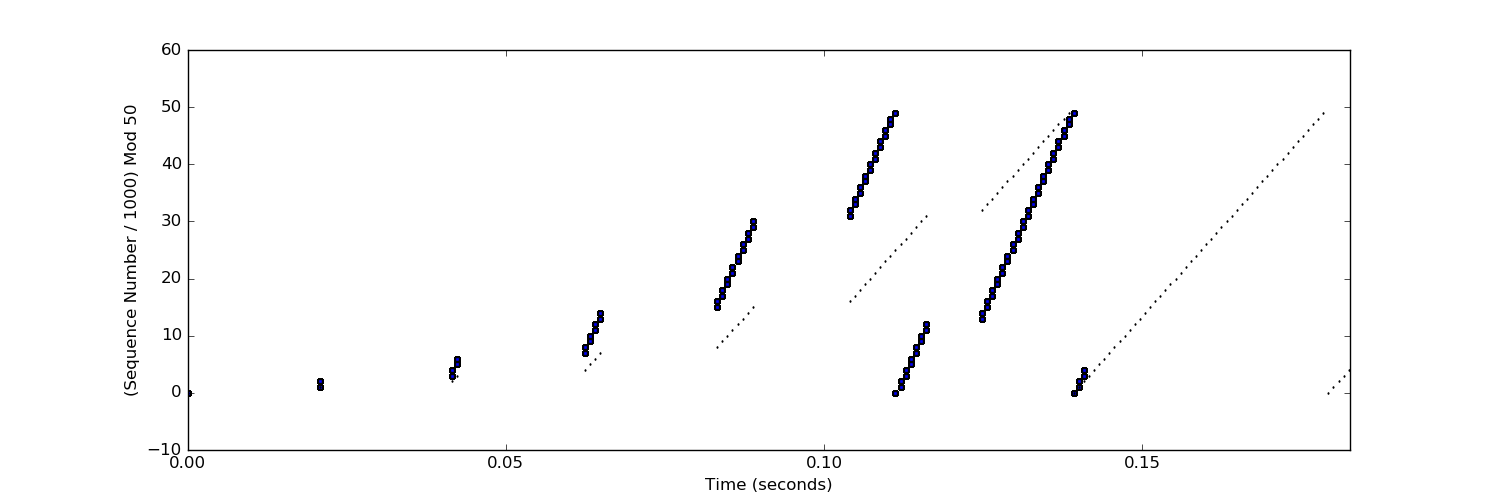
\includegraphics[width=\linewidth]{figure1}
\end{figure}

%discuss slow start here
The purpose of this test was to demonstrate that slow start worked correctly. A small file (about 100 KB) was transfered with 0 packet loss. The file transfer began with a window size of 1,000 bytes and a threshold of 100,000 bytes where the maximum packet size was 1,000 bytes. For this test the entire file was transfered within the slow start period. As show in Figure 1, our implementation of slow start works correctly in this case because for each ACK recieved there are two new packets sent. This results in an expontentially growing window size. 
\bigskip
  \item Additive Increase
  
  \begin{figure}[H]
\caption{The graph of our additive increase test output.}
	\label{figure2}
  	\centering
  	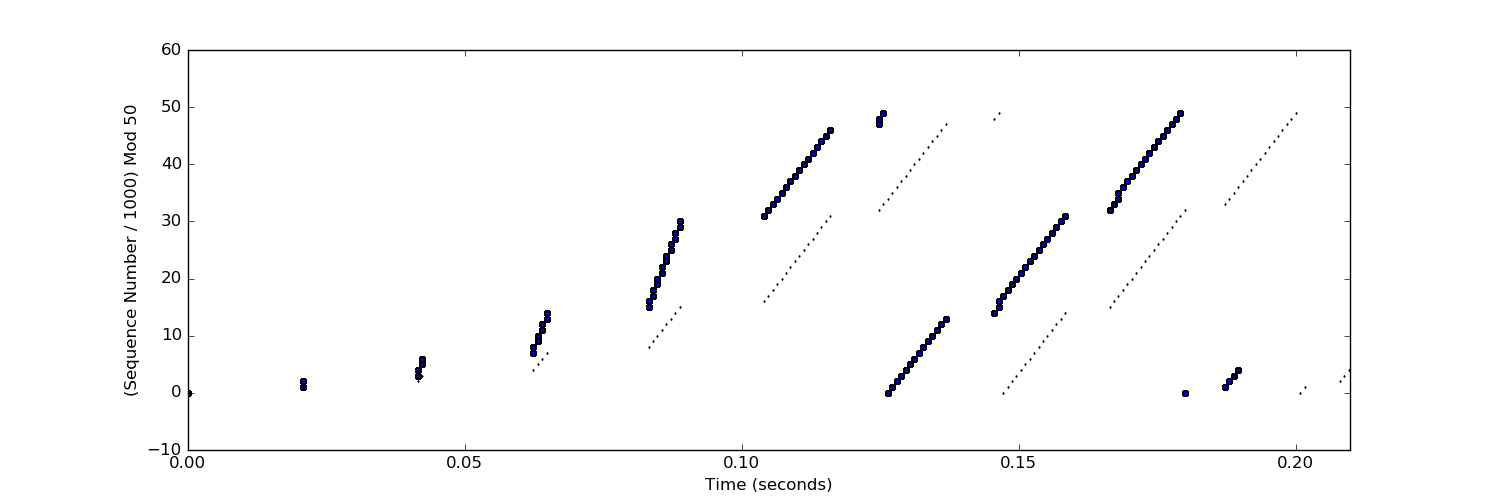
\includegraphics[width=\linewidth]{figure2}
\end{figure}

%discuss additive increase here
The purpose of this test was to demonstrate that slow start transitions to additive increase correctly once the window size hits the slow start threshold. Again, a small file (about 100 KB) was transfered with 0 packet loss. The file transfer began with a window size of 1,000 bytes and a threshold of 16,000 bytes where the maximum packet size was 1,000 bytes. We can see by looking at the packet groupings in Figure 2 that additive increase does take over from slow start when the window size reaches 16,000 bytes. The first 5 groupings of packets happen during slow start. As expected, the groups double in size as they progress (1, 2, 4, 8, 16). The subsequent groupings increase by one packet in each grouping (16, 17, 18, 19), which shows that the window size is increasing by 1000 bytes rather than doubling.
\bigskip
  \item AIMD

\begin{figure}[H]
\caption{The graph of our AIMD test output.}
	\label{figure3}
  	\centering
  	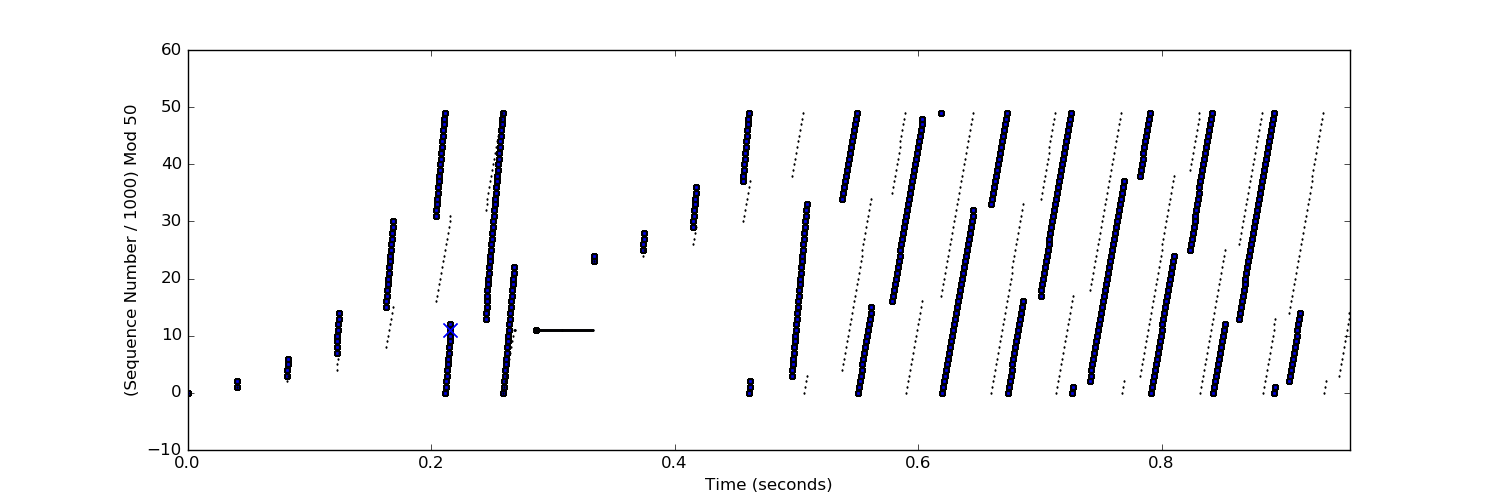
\includegraphics[width=\linewidth]{figure3}
\end{figure}

%discuss AIMD here
The purpose of this test was to demonstrate that once loss occurs TCP restarts slow start up to a smaller threshold and then continues. A medium sized file (about 500 KB) was transfered with a loss event happening at the end of the window once the window size became 32 packets. The file transfer began with a window size of 1,000 bytes and a threshold of 100,000 bytes. 

As shown in Figure 3, our implementation of loss handling is correct in this case for the several reasons. Once TCP slow starts to a window of 32 packets, it has a loss event as indicated by the blue X. The sender quickly receives 3 duplicate ACKs for the lost packet, at which time fast retransmit comes into effect. Fast retransmit is indicated by the single packet sent at the beginning of the line of ACKs for the same sequence number at about 0.15 seconds. This results in just the single lost packet being immedietely resent and then waiting for that packet to be ACKed (which it is shortly thereafter). Once the retransmitted packet is ACKed, transmission continues normally by using slow start with a smaller threshold. Once this threshold is reached, transmission uses additive increase.
\bigSkip
  \item Burst Loss

\begin{figure}[H]
\caption{The graph of our burst loss test output.}
	\label{figure4}
  	\centering
  	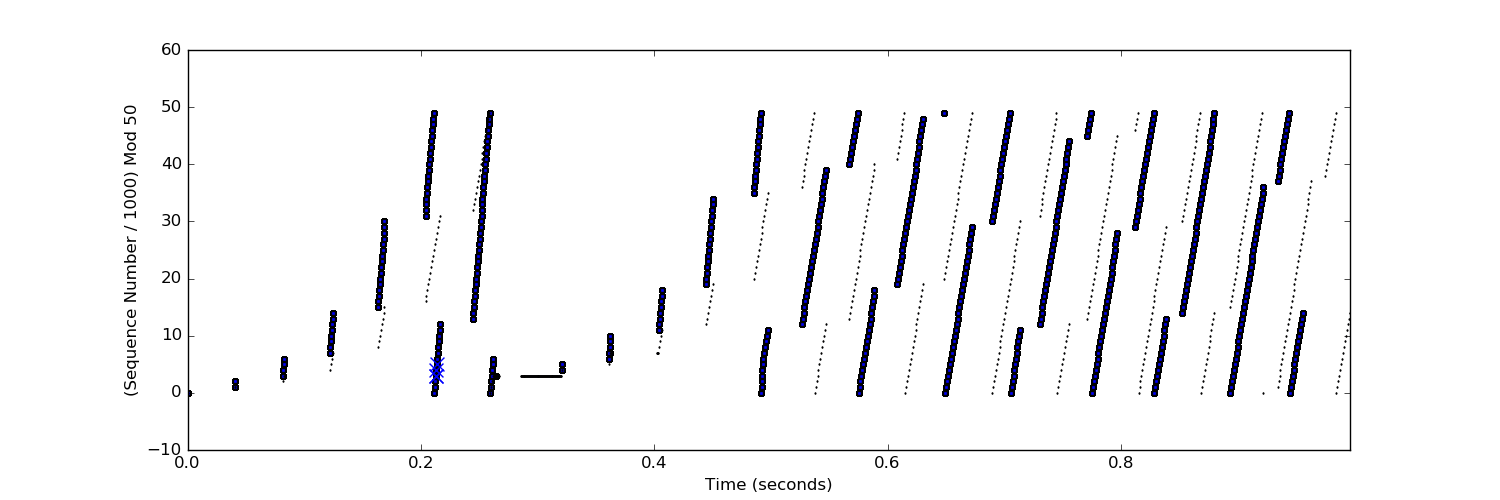
\includegraphics[width=\linewidth]{figure4}
\end{figure}

%discuss burst loss
The purpose of this test was to demonstrate that TCP resets to slow start and recovers normally when we have three consecutive loss events. A medium sized file (about 500 KB) was transfered with three consecutive loss events in the first grouping when the window size was 32 packets. It began with a window size of 1,000 bytes and a threshold of 100,000 bytes.

Figure 4 shows that our implementation handles burst loss as expected. When 3 consective packets are lost, 3 duplicate ACKs are received for the first lost packet. At that time, fast retransmit causes the first lost packet to be retransmitted which is shown by the single transmitted packet towards the beginning of the line of duplicate ACKs. The retransmitted packet is ACKd with a request for the second dropped packet, which is sent and initiates slow start again with a smaller threshhold. We can see that Figure 4 looks very similar to Figure 3 which is to be expected because the method for handling 1 lost packet vs 3 lost packets is nearly identical.


\end{enumerate}


\end{document}
